\documentclass[a4paper,10pt]{article}
\usepackage[utf8]{inputenc}
\usepackage[T1]{fontenc}
\usepackage{lmodern}	
\usepackage[italian]{babel}

\usepackage{amsmath}
\usepackage{amsfonts}
\usepackage{amssymb}

\usepackage{graphicx}
\usepackage[dvipsnames]{xcolor}  %colori

\usepackage[left=2cm,right=2cm,top=2cm,bottom=2cm]{geometry}
\geometry{a4paper}

\usepackage{verbatim}

\usepackage{booktabs}
\usepackage{subfig}
\usepackage{float}

\usepackage[colorlinks=true, linkcolor=black, urlcolor=blue, citecolor=darkgray, filecolor=darkgray]{hyperref}   %per gli hyperlink
\usepackage[italian, sort, noabbrev, capitalise]{cleveref}
\usepackage[bottom]{footmisc}

\usepackage[cdot, thickqspace, squaren]{SIunits}
% macro
\def\code#1{\texttt{#1}}

\title{Esercitazione 14: Misura della costante di assorbimento del mylar\\ usando un
	amplificatore lock-in}
\author{Gruppo BL \\ Candido Alessandro, Luzio Andrea, Mazziotti Fabrizio}

\begin{document}

\maketitle

\section{Scopo e Strumentazione}
In questa esercitazione si vuole effettuare una misura di assorbimento della luce di uno spessore di mylar facendo uso di un amplificatore sincrono sensibile alla fase, o lock-in.
\newline

\noindent La strumentazione è quella solitamente presente sul banco di lavoro, e inoltre si è usato:
\begin{itemize}
	\item TL082: JFET input dual op-amp (x1);
	\item TL081: JFET input op-amp (x4);
	\item SN7400: quad NAND gates;
	\item DG441: quad CMOS analog switch;
	\item 2N1711, BC182: NPN transistors;
	\item LED rosso; fotodiodo.
\end{itemize}

Lo schema a blocchi del circuito è riportato in 

\begin{figure}[H]
	\centering
	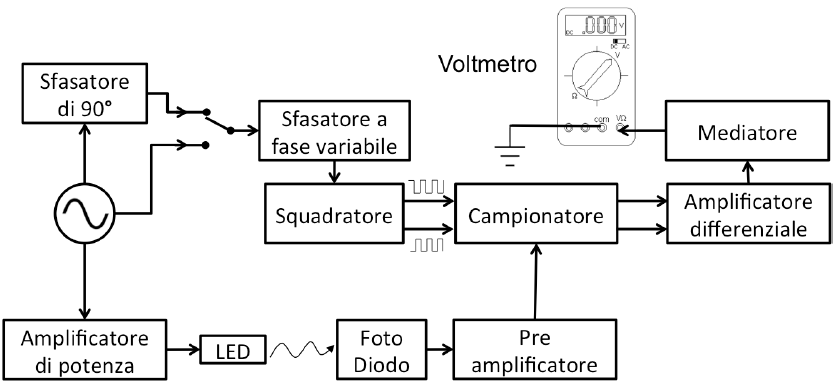
\includegraphics[width=\textwidth]{../grafici/Blocks.png}
	\caption{Schema a blocchi del circuito complessivo}
	\label{fig:blocks}
\end{figure}

\section{Implementazione dei blocchi di circuito}

\subsection{Amplificatore di potenza}

\subsection{Preamplificatore}

\subsection{Sfasatore di $90^\circ$}

\begin{figure}[H]
	\centering
	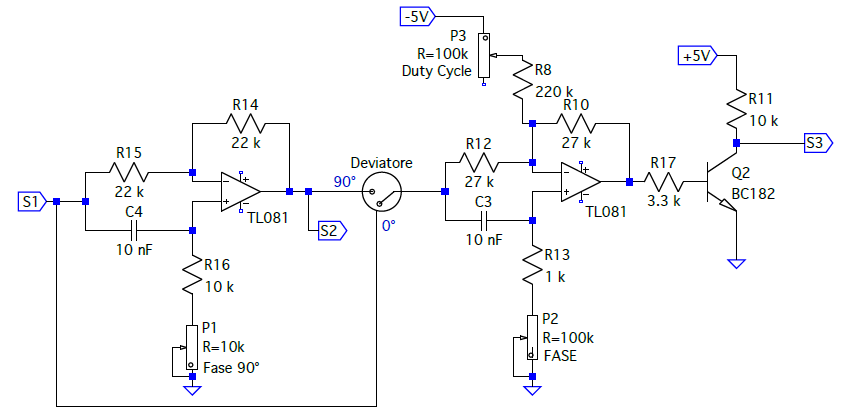
\includegraphics[width=\textwidth]{../grafici/Dephaser.png}
	\caption{Schema del circuito: sfasatore di $90^\circ$ e sfasatore a fase variabile.}
	\label{fig:deph}
\end{figure}

\subsection{Sfasatore a fase variabile}

\subsection{Squadratore e campionatore}

\subsection{Amplificatore differenziale}

\subsection{Mediatore}

\section{Misure di assorbimento}

\end{document}